\documentclass{article}
\usepackage[usenames,dvipsnames]{color}
\usepackage{amssymb,amsmath, multirow}
\usepackage[initials]{amsrefs}
\usepackage{fullpage}
%\usepackage[all]{xy}
\usepackage{mathrsfs} %% for \mathscr and \mathfrak
\usepackage{graphicx} %% for \includegraphics
\usepackage{float}
\usepackage[pdftex,plainpages=false,hypertexnames=false,pdfpagelabels]{hyperref}
\usepackage{xcolor}
\definecolor{dark-red}{rgb}{0.7,0.25,0.25}
\definecolor{dark-blue}{rgb}{0.15,0.15,0.55}
\definecolor{medium-blue}{rgb}{0,0,0.65}
\hypersetup{
  colorlinks, linkcolor={purple},
  citecolor={medium-blue}, urlcolor={medium-blue}
}

%\theoremstyle{hharemark}
\newtheorem{theorem}{Theorem}[section]
\newtheorem{proposition}[theorem]{Proposition}
\newtheorem{lemma}[theorem]{Lemma}
\newtheorem{corollary}[theorem]{Corollary}
\newtheorem{definition}[theorem]{Definition}
\newtheorem{assumption}[theorem]{Assumption}
\newtheorem{remark}{Remark}

\def\R{\mathbb{R}}
\def\Z{\mathbb{Z}}
\def\ds{\displaystyle}
\def\der#1#2{\frac{\partial #1}{\partial #2}} % partial derivatives
\def\d#1#2{\frac{d#1}{d#2}} % standard derivatives
\def\dt#1#2{\frac{d^2#1}{d#2^2}}
\def\dth#1#2{\frac{d^3#1}{d#2^3}}
\def\com#1{\texttt{#1}}
\def\x{\mathbf{x}}
\def\v{\mathbf{v}}
\def\bpm{\begin{pmatrix}}
\def\epm{\end{pmatrix}}
\def\O{\mathcal{O}}
\newcommand{\checked}{\makebox[0pt][l]{$\checkmark$}$\square$}
\newcommand{\unchecked}{$\Box$}
%\Theoremstyle{remark}
\DeclareMathOperator\erfc{erfc}
\DeclareMathOperator\erf{erf}
% Bernard Deconinck's macros
\newcommand{\beq}{\begin{equation}}
\newcommand{\eeq}{\end{equation}}
\newcommand{\ba}{\begin{array}}
\newcommand{\ea}{\end{array}}
\newcommand{\bea}{\begin{eqnarray*}}
\newcommand{\eea}{\end{eqnarray*}}
\newcommand{\bc}{\begin{center}}
\newcommand{\ec}{\end{center}}
\newcommand{\bt}{\begin{table}}
\newcommand{\et}{\end{table}}
\newcommand{\la}[1]{\label{#1}}
\newcommand{\p}{\partial}
\newcommand{\pp}[2]{{\partial #1 \over \partial #2}}
\newcommand{\ppn}[3]{{\partial^{#1} #2 \over \partial #3^{#1}}}
\newcommand{\mbf}[1]{\mbox{\boldmath {$#1$}}}
\newcommand{\red}[1]{\textcolor{red}{#1}}
\newcommand{\green}[1]{\textcolor{green}{#1}}
\newcommand{\blue}[1]{\textcolor{blue}{#1}}
\newcommand{\yellow}[1]{\textcolor{yellow}{#1}}
\newcommand{\purple}[1]{\textcolor{purple}{#1}}
\newcommand{\black}[1]{\textcolor{black}{#1}}
\usepackage{url}

\DefineSimpleKey{bib}{myurl}

\newcommand\myurl[1]{\url{#1}}

\BibSpec{webpage}{%
  +{}{\PrintAuthors} {author}
  +{,}{ \textit} {title}
  +{}{ \parenthesize} {date}
  +{,}{ \myurl} {myurl}
  +{,}{ } {note}
  +{.}{ } {transition}
}

\begin{document}
\begin{titlepage}
  \begin{center}
    \bfseries
\huge Mastering \\ The Black-Scholes Equation \\[.5in]
\vfill
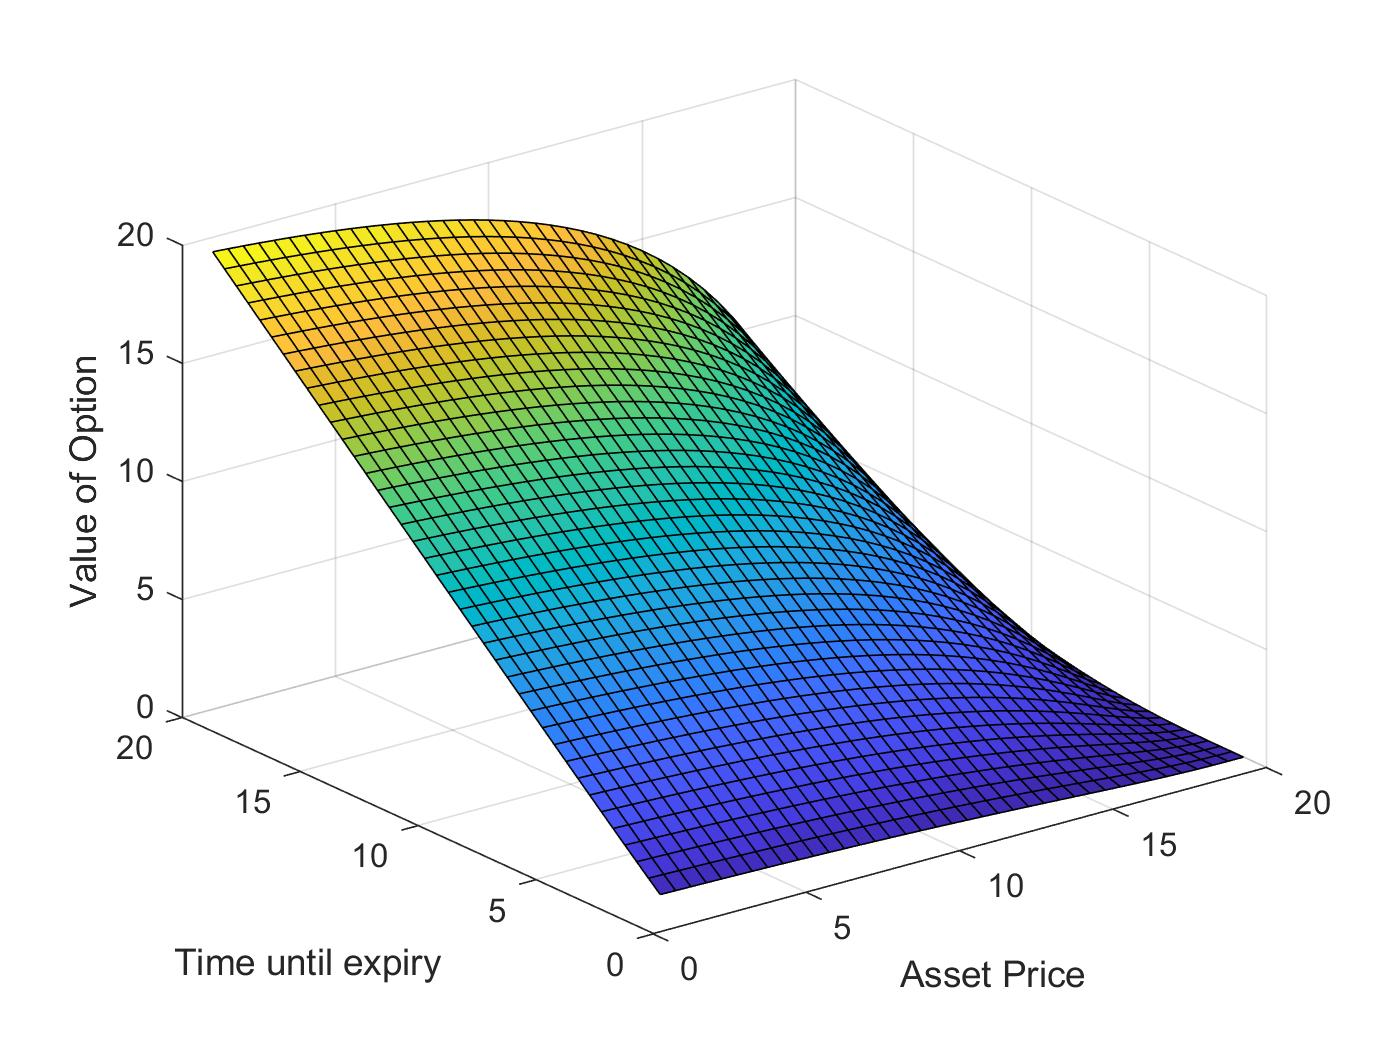
\includegraphics[height=3.5in]{BlackScholes3D}
\vfill
\LARGE Brennan Reamer \\[.2in]
\texttt{reamerb1@wit.edu}\\
\texttt{December 2020}
\end{center}      
\end{titlepage}
\newpage
\section{The Black-Scholes Equation}
\subsection{Introduction}
The Black-Scholes Equation is very useful in economics. It is able to provide the value of a single option based on the volatility of the asset, the fixed interest rate, the exercise price, and the time until expiration. The Black-Scholes Equation assumes the following to be true, \cite{notes}:
\begin{itemize}
\item{The asset price follows geometric Brownian motion.}
\item{The risk-free interest rate $r$ is known.}
\item{The asset volatility $\sigma$ is known.}
\item{The asset does not pay dividends.}
\item{There are no transaction costs.}
\item{The option cannot be sold before its expiry (ie. it is a European option).}
\end{itemize}
\subsection{Derivation}
\bea
\pp{u}{t}+\frac{\sigma^2}{2} x^2 \ppn{2}{u}{x}+rx\pp{u}{x}-ru &=& 0
\eea
The dependent variable $u(t,x)$ represents the value of a single option, a contract to either buy or sell at an exercise price $p$ at a future time $t_*$.
The constant $\sigma>0$ represents the asset's volatility. $r$ is the fixed interest rate for bank deposits, where a return is guaranteed instead of buying the option. Borrowed money is indicated by a negative value of $r$.\\\\
The Black-Scholes equation is a backwards diffusion process as the diffusion term $u_{xx}$ in the following equation has a negative coefficient, \cite{textbook}.
\bea
u_t &=& -\frac{\sigma^2}{2} x^2 u_{xx} -rxu_x +ru
\eea
In order to evaluate the equation, we need to determine the option's value $u(t,x)$ at the current time $t$ and asset value $x$. For a European call option, the asset is bought at the exercise price $p>0$ at the specified time and the final condition may be written as
\bea
u(t_*,x) &=& \max\{x-p,0\},
\eea
representing a profit when $x>p$, or the option not being exercised at $x\leq p$ to avoid a loss. For a European put option, the asset is sold and the final condition may be written as
\bea
u(t_*,x) &=& \max\{p-x,0\}.
\eea
The solution $u(t,x)$ is defined for all $t<t_*$ and $x>0$ subject to the boundary conditions
\bea
u(t,0) = 0, & u(t,x) \sim x & \text{as  }  x \rightarrow \infty.
\eea
The ratio $\frac{u(t,x)}{x}$ tends to a constant as $x \rightarrow \infty$.\\
\subsection{Solving the Black Scholes Equation}
The Black-Scholes equation may be solved explicitly by transforming it into the heat equation, \cite{textbook}. The first step is to convert it to a forward diffusion process:\\
\bea
\tau = \frac{1}{2} \sigma^2(t_*-t), & v(\tau, x) = u(t_*-2\frac{\tau}{\sigma^2}, x)
\eea
where $\tau$ runs forward from 0 as the actual time $t$ runs backwards from $t_*$. This converts the final condition into an initial condition $v(0,x) = f(x)$. $v(\tau,x)$ satisfies
\bea
\pp{v}{\tau} = x^2 \ppn{2}{v}{x}+\kappa x\pp{v}{x}-\kappa v, & \text{where} & \kappa = \frac{2r}{\sigma^2}.
\eea
A change of variables using $x = e^y$ can then take place to remove the explicit dependence on the independent variable $x$.
\bea
\omega(\tau, y) =& v(\tau, e^y) &= v(\tau, x)
\eea
The following derivatives can be computed from above.
\bea
\pp{\omega}{\tau} &=& \pp{v}{\tau}\\
\pp{\omega}{y} &=& e^y\pp{v}{x} = x\pp{v}{x}\\
\ppn{2}{\omega}{y} &=& e^{2y}\ppn{2}{v}{x} + e^y\pp{v}{x} = x^2\ppn{2}{v}{x} + x\pp{v}{x}
\eea
We can use $\omega$ to solve the partial differential equation
\bea
\pp{\omega}{\tau} &=& \ppn{2}{\omega}{y} + (\kappa-1)\pp{\omega}{y} - \kappa \omega.
\eea
The heat equation can be found by setting
\bea
\omega(\tau, y) &=& e^{\alpha \tau+\beta y}z(\tau, y),
\eea
where $\alpha$ and $\beta$ are constants. Substituting into the previous equation gives us
\bea
\pp{z}{\tau} + \alpha z &=& \ppn{2}{z}{y} +2\beta\pp{z}{y} + \beta^2 z+(\kappa-1)\left(\pp{z}{y}+\beta z\right) - \kappa z.
\eea
The terms involving $z$ and $\pp{z}{y}$ can be eliminated by setting
\bea
\alpha = -\frac{1}{4} (\kappa+1)^2, & \beta = -\frac{1}{2} (\kappa-1).
\eea
In conclusion, the heat equation,
\bea
\pp{z}{\tau} &=& \ppn{2}{z}{y},
\eea
can be satisfied by the function
\bea
z(\tau,y) &=& e^{\frac{1}{4}(\kappa+1)^2\tau+\frac{1}{2}(\kappa-1)y}\omega(\tau, y).
\eea
So far, we have discovered that for $\tau > 0, -\infty < y < \infty$,
\begin{eqnarray}\label{sol1}
u(t,x) &=& x^{-\frac{1}{2}(\kappa-1)}e^{-\frac{1}{8}(\kappa+1)^2\sigma^2(t_*-t)}z\left(\frac{1}{2}\sigma^2(t_*-t), \log x\right)
\end{eqnarray}
solves the final value problem for the Black-Scholes Equation for $t<t_*$ and $0<x<\infty$.\\\\
The solution to the initial value problem can be written as
\bea
z(\tau,y) &=& \frac{1}{2\sqrt{\pi\tau}}\int_{-\infty}^{\infty}{e^{-\frac{(y-\eta)^2}{4\tau}+\frac{(\kappa-1)\eta}{2}}f(e^\eta)d\eta}.
\eea
This can be combined with (\ref{sol1}) to produce an explicit solution formula for the general final value problem for the equation.
\subsection{European Call Option}
The initial condition,\\
\bea
z(0,y) = h(y) &=& e^{\frac{(\kappa-1)y}{2}}\max\{e^y-p, 0\},
\eea
results in the integral
\bea
z(\tau,y) &=& \frac{1}{2\sqrt{\pi\tau}}\int_{\log{p}}^{\infty}{e^{-\frac{(y-\eta)^2}{4\tau}+\frac{(\kappa-1)\eta}{2}}(e^\eta-p)d\eta}.
\eea
The integral can be evaluated to produce
\bea
z(\tau,y) &=& \frac{1}{2}\left[e^{\frac{(\kappa+1)^2\tau}{4}+\frac{(\kappa+1)y}{2}}\erfc\left(\frac{\log{p}-(\kappa+1)\tau-y}{2\sqrt{\tau}}\right)-pe^{\frac{(\kappa-1)^2\tau}{4}+\frac{(\kappa-1)y}{2}}\erfc\left(\frac{\log{p}-(\kappa-1)\tau-y}{2\sqrt{\tau}}\right)\right],
\eea
where $\erfc(x)$ is the complementary error function, or
\bea
\erfc(x) &=& \frac{2}{\sqrt{\pi}}\int_{x}^{\infty}{e^{-z^2}dz} = 1-\erf(x).
\eea
Plugging this back into (\ref{sol1}) results in the Black-Scholes Formula for a European call option:\\
\bea\boxed{
u(t,x) = \frac{1}{2}\left[x\erfc\left(-\frac{(r+\frac{1}{2}\sigma^2)(t_*-t)+\log(\frac{x}{p})}{\sqrt{2\sigma^2(t_*-t)}}\right)-pe^{-r(t_*-t)}\erfc\left(-\frac{(r-\frac{1}{2}\sigma^2)(t_*-t)+\log(\frac{x}{p})}{\sqrt{2\sigma^2(t_*-t)}}\right)\right].
}
\eea
An example of this in use is shown in Figure \ref{fig:solution} with the input values of $t_* = 10$, $r = .08$, $\sigma = .82$, and $p = 25$.\\
\begin{figure}[H]
\begin{center}
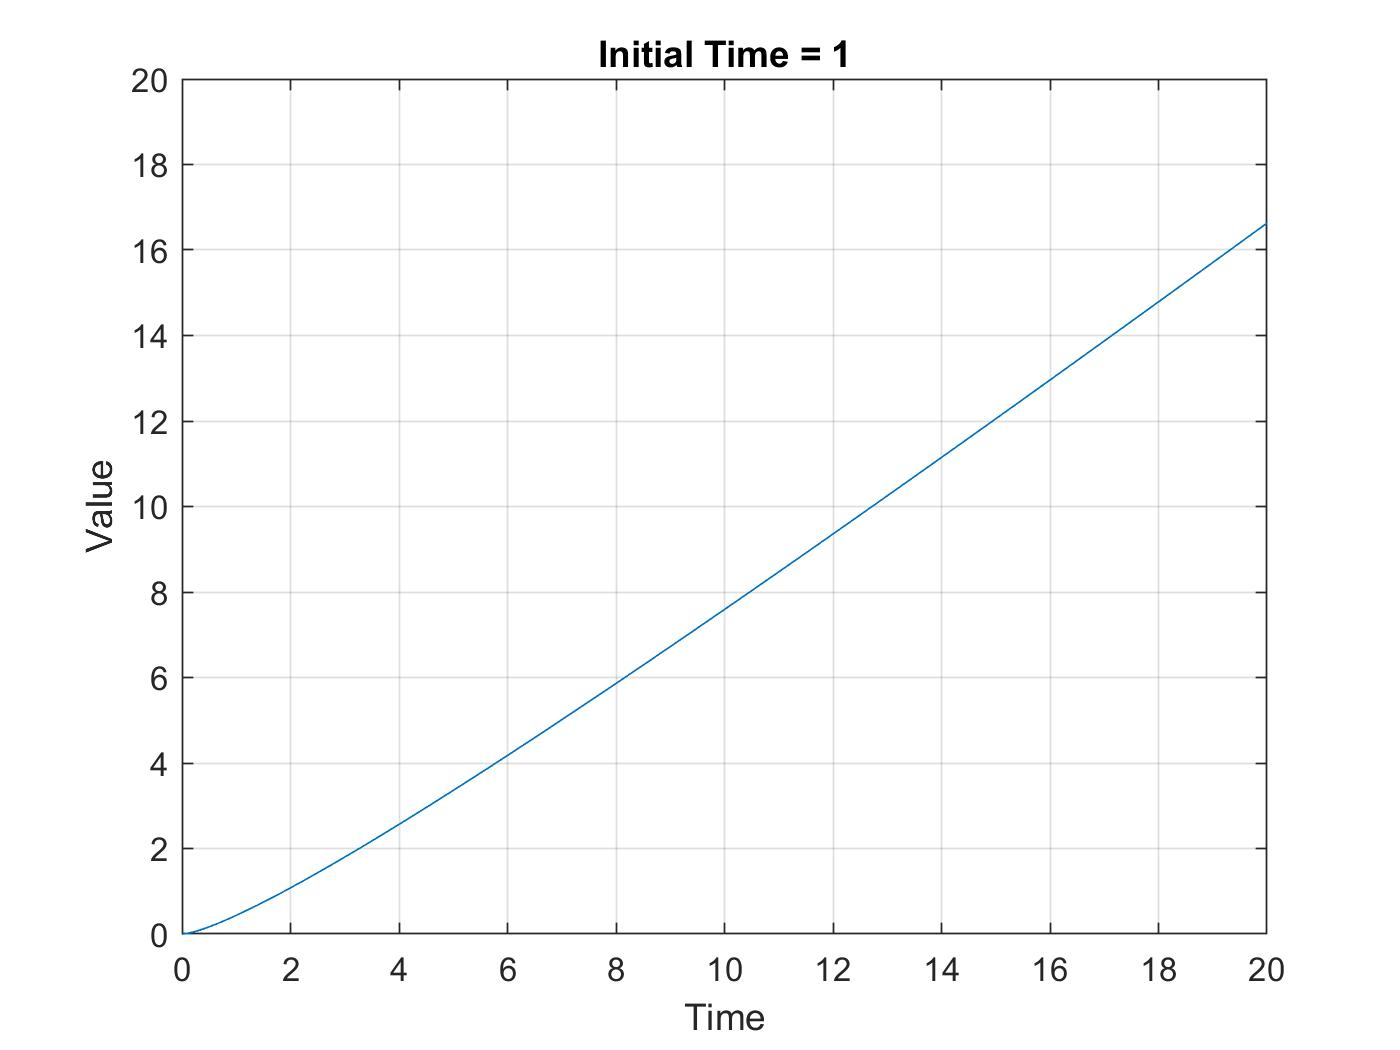
\includegraphics[height = 1.5 in]{t1.10}
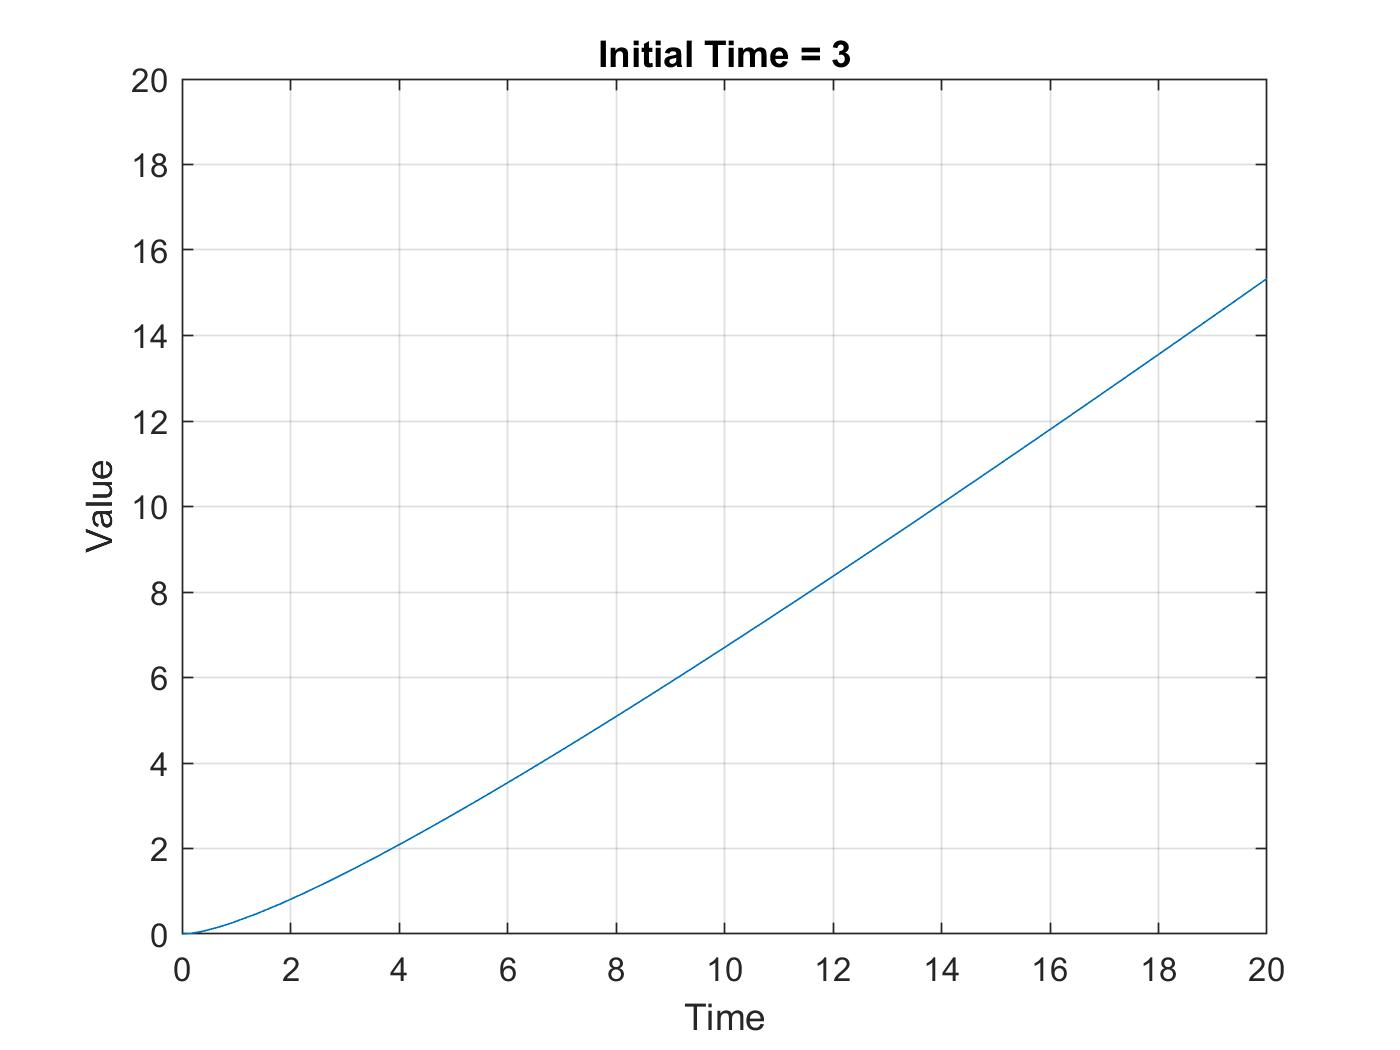
\includegraphics[height = 1.5 in]{t3.10}
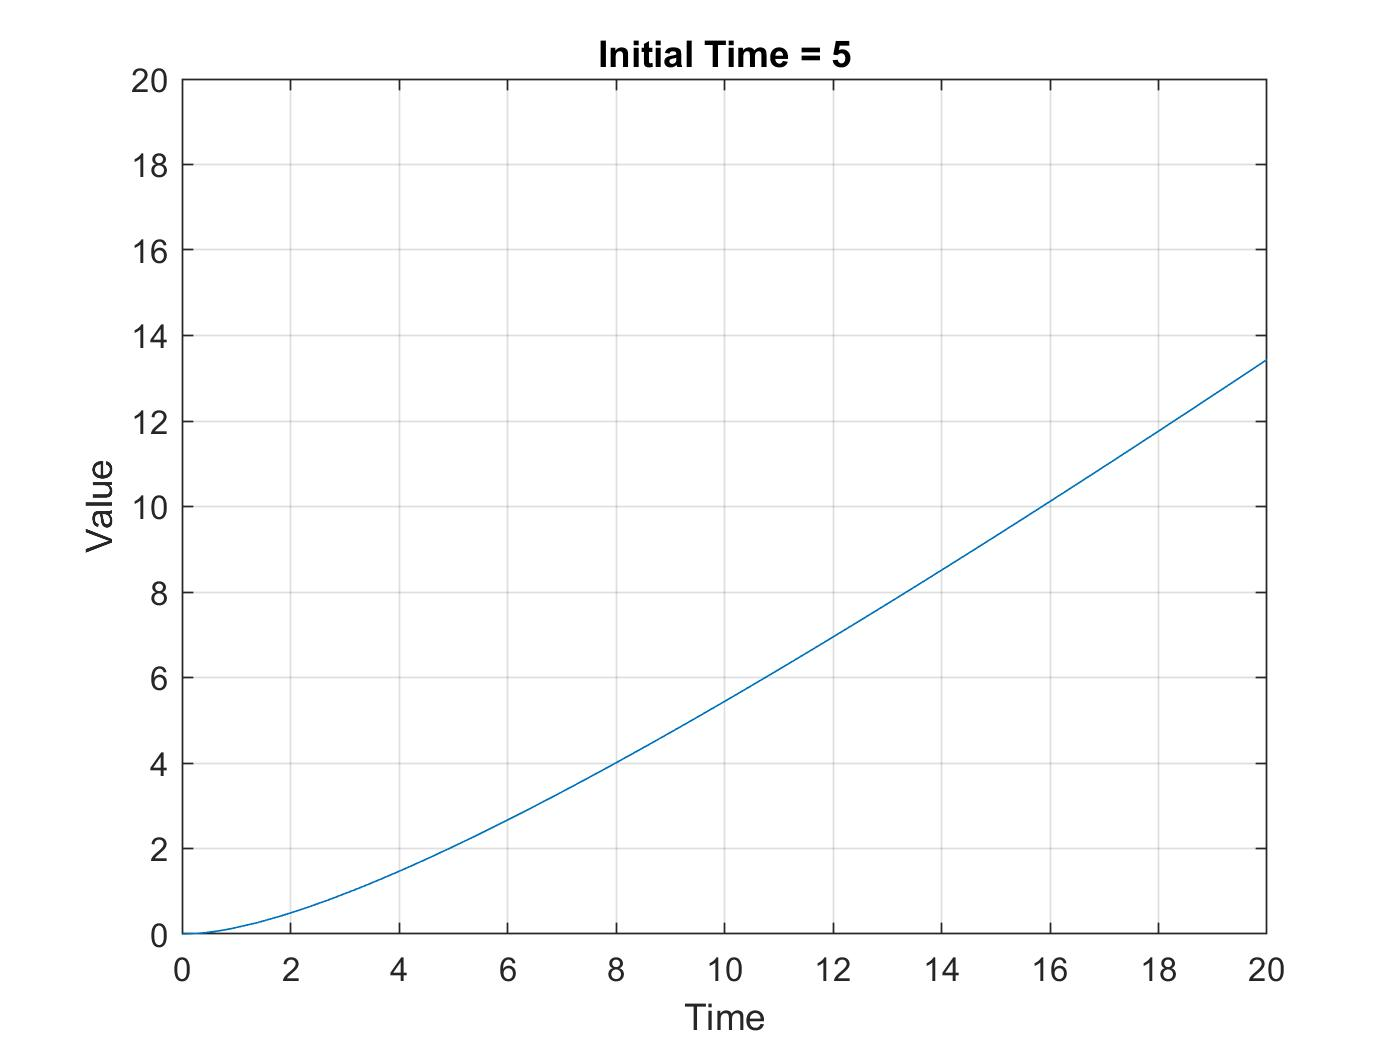
\includegraphics[height = 1.5 in]{t5.10}\\
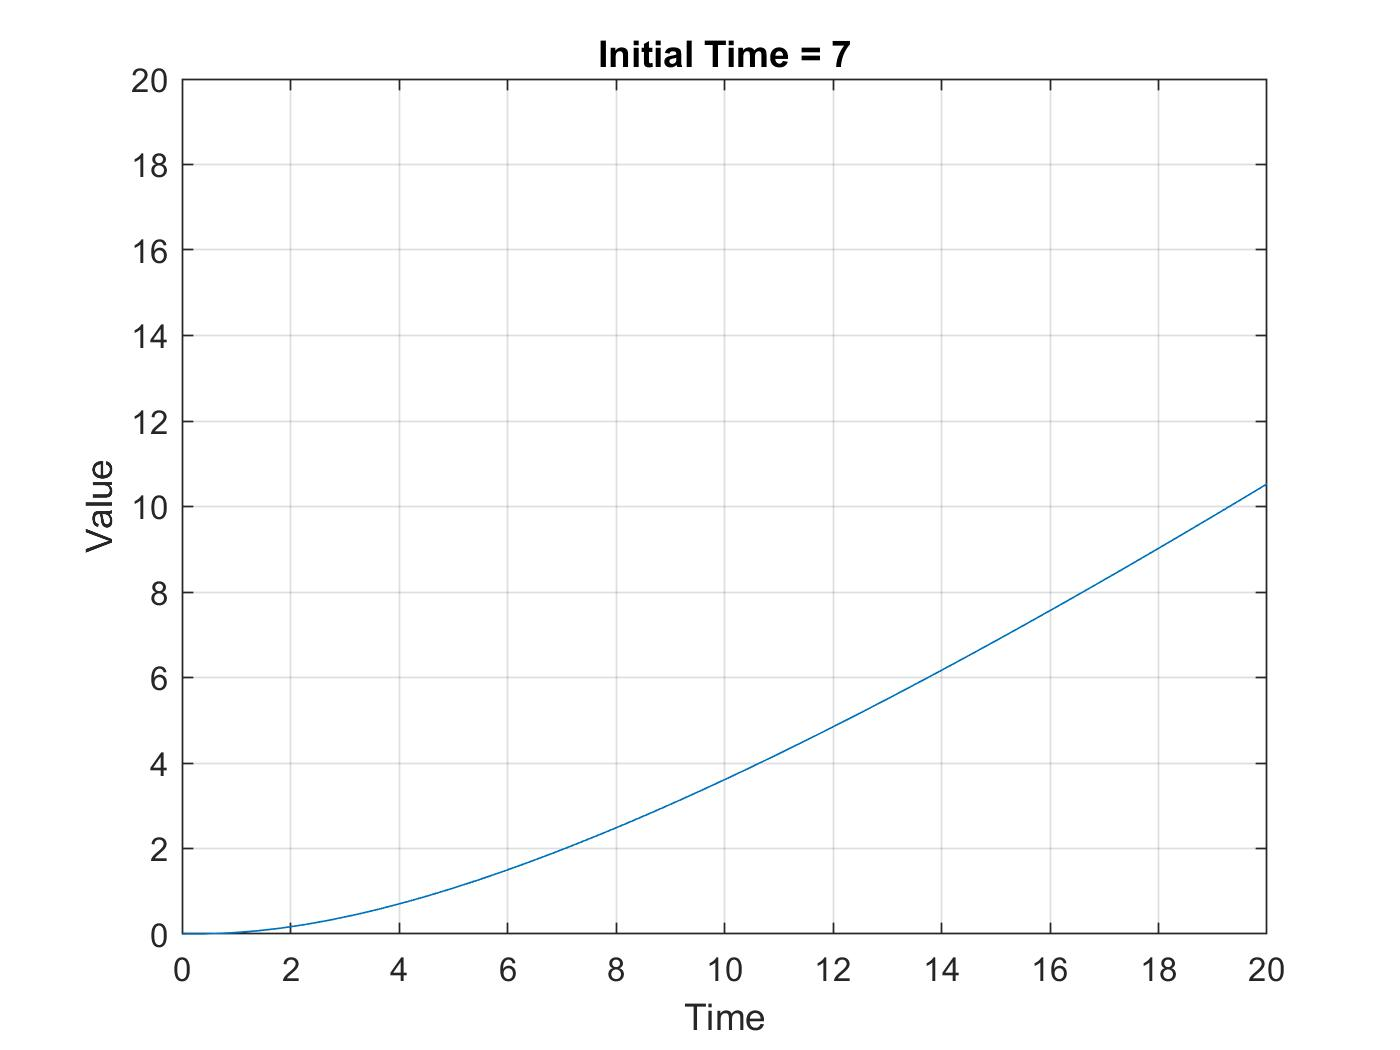
\includegraphics[height = 1.5 in]{t7.10}
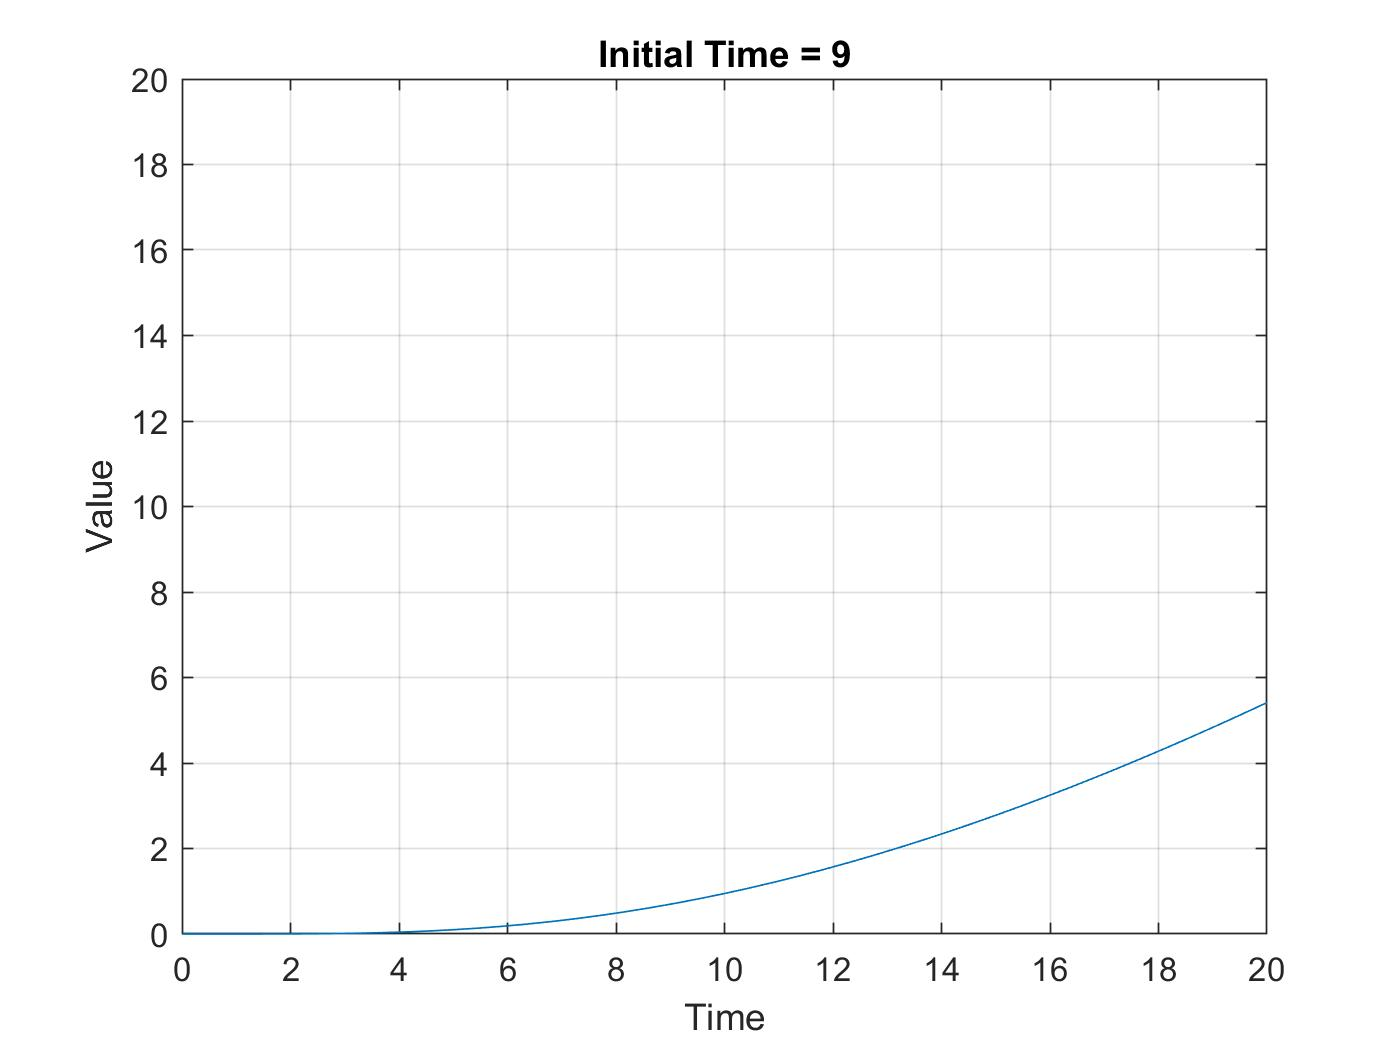
\includegraphics[height = 1.5 in]{t9.10}
\caption{Graphs to the Solution of the Black-Scholes equation \label{fig:solution}}
\end{center}
\end{figure}
The option's value decreases as the time gets closer to the exercise time $t_*$, lessening the chances of profit from the asset's remaining volatility.
\section{Matlab Implementation}
The Black-Scholes Equation can be implemented using Matlab for ease of calculation. Below are two Matlab programs, one solves the Black-Scholes Equation numerically and the other creates a graph of the solution.
\subsection{Numerical Solution}
The following code outputs the value of the asset according to the Black-Scholes Equation depending on the inputs $t_*$, $\sigma$, $r$, $p$, $t$, and $x$.
\begin{verbatim}
function u = BlackScholesEq(t_final, sigma, r, p, t, x)
% Computes the value of a European call option at expiration

%Inputs:
%t_final = Time until expiry
%sigma = Volatility of asset
%r = Fixed Interest Rate
%p = Exercise Price of asset
%t = initial time (usually 0)
%x = asset price at initial time

u = (1/2)*(x*erfc(-((r+0.5*sigma^2)*(t_final-t)+log(x/p))/(sqrt(2*sigma^2*(t_final-t))))-p*exp(-r*(t_final-t))*erfc(-((r-0.5*sigma^2)*(t_final-t)+log(x/p))/(sqrt(2*sigma^2*(t_final-t)))));
\end{verbatim}
\subsection{Graphical Solution}
The second way to implement the equation using Matlab consists of graphing the output of the Black-Scholes Equation with respect to time until expiration. Examples of this program's output can be seen in Figure \ref{fig:solution}. It can be seen that as initial time $T$ progresses, the value of the asset decreases as time gets closer to the exercise time $t_{final}$. The function is dependent on the inputs $t_*$, $\sigma$, $r$, $p$, and $T$.
\begin{verbatim}
function u = BSGrph(t_final, sigma, r, p, T)
% Graphs the value of a European call option in respect to time until expiration

%Inputs:
%t_final = Time until expiry
%sigma = Volatility of asset
%r = Fixed Interest Rate
%p = Exercise Price of asset
%T = Initial Time (Requirement: T < t_final)

syms x t
u(t,x) = (1/2)*(x*erfc(-((r+0.5*sigma^2)*(t_final-t)+log(x/p))/(sqrt(2*sigma^2*(t_final-t))))-p*exp(-r*(t_final-t))*erfc(-((r-0.5*sigma^2)*(t_final-t)+log(x/p))/(sqrt(2*sigma^2*(t_final-t)))));
fplot(u(T,x))
grid
xlim([0 20])
ylim([0 20])
title(['Initial Time = ', num2str(T)])
xlabel('Time')
ylabel('Value')
\end{verbatim}
\section{Downfalls of the Black-Scholes Equation}
While being a popular equation used to model stock options and allowing one to trade without risk, the Black-Scholes Equation has its downfalls, \cite{brilliant}. There are numerous criticisms on its ability to accurately reflect the market:
\begin{itemize}
\item Returns do not absolutely follow a normal distribution. They tend to be leptokurtic, or more concentrated about the mean with fat tails.
\item A risk-free interest rate is assumed in the calculations of the solution, but it is not possible to calculate an exactly risk-free rate. Investors tend to use the long-term yield of bonds as risk-free interest rates, but they are not truly risk-free. They are simply the least risky investment according to the market.
\item The Black-Scholes model assumes a market using European options, where the asset cannot be sold until its expiry. Most options traded today are American options, where the asset can be sold at any point.
\end{itemize}
\bibliography{blackscholes}
\nocite{*}
\end{document}